\begin{frame} \frametitle{Autonomous Underwater Vehicle (AUV)}
\vspace{-25pt}
\begin{columns}[t]
	\column{.55\textwidth}
%	\begin{block}{Nessie AUV (Ocean Systems Lab, UK)}
	\begin{block}{Sensors}	
	$\bullet$ Pressure sensor: depth  \\
	\pro {\footnotesize precise absolute depth} \\
	$\bullet$ Digital compass: 3d attitude  \\
	\contra {\footnotesize magnetic declination}
	\contra {\footnotesize prone to disturbances}
	\pro {\footnotesize absolute measurement} \\
	$\bullet$ Fibre-optic gyro: orientation rate \\
	\pro {\footnotesize high accuracy} \\
	%\contra {\footnotesize relative measurement} \\
	$\bullet$ Doppler Velocity Log (DVL): 3d speed vector, altitude \\
	\contra {\footnotesize needs certain altitude to work} 
	\end{block}
	%\begin{itemize}	
	$\bullet$ GPS: latitude, longitude  \\  
	\contra {\footnotesize only on the surface} \\
	$\bullet$ Long-baseline (LBL): absolute 3d position - north, east, depth	
	%\end{itemize}

%	\end{block}
	\column{.42\textwidth}
	\centering

	\begin{block}{Platform: Nessie AUV}
	\centering
	\includegraphics[width=0.8\linewidth]{fig/nessie.pdf}
	\end{block}

	\begin{block}{Absolute positioning}
	\centering
	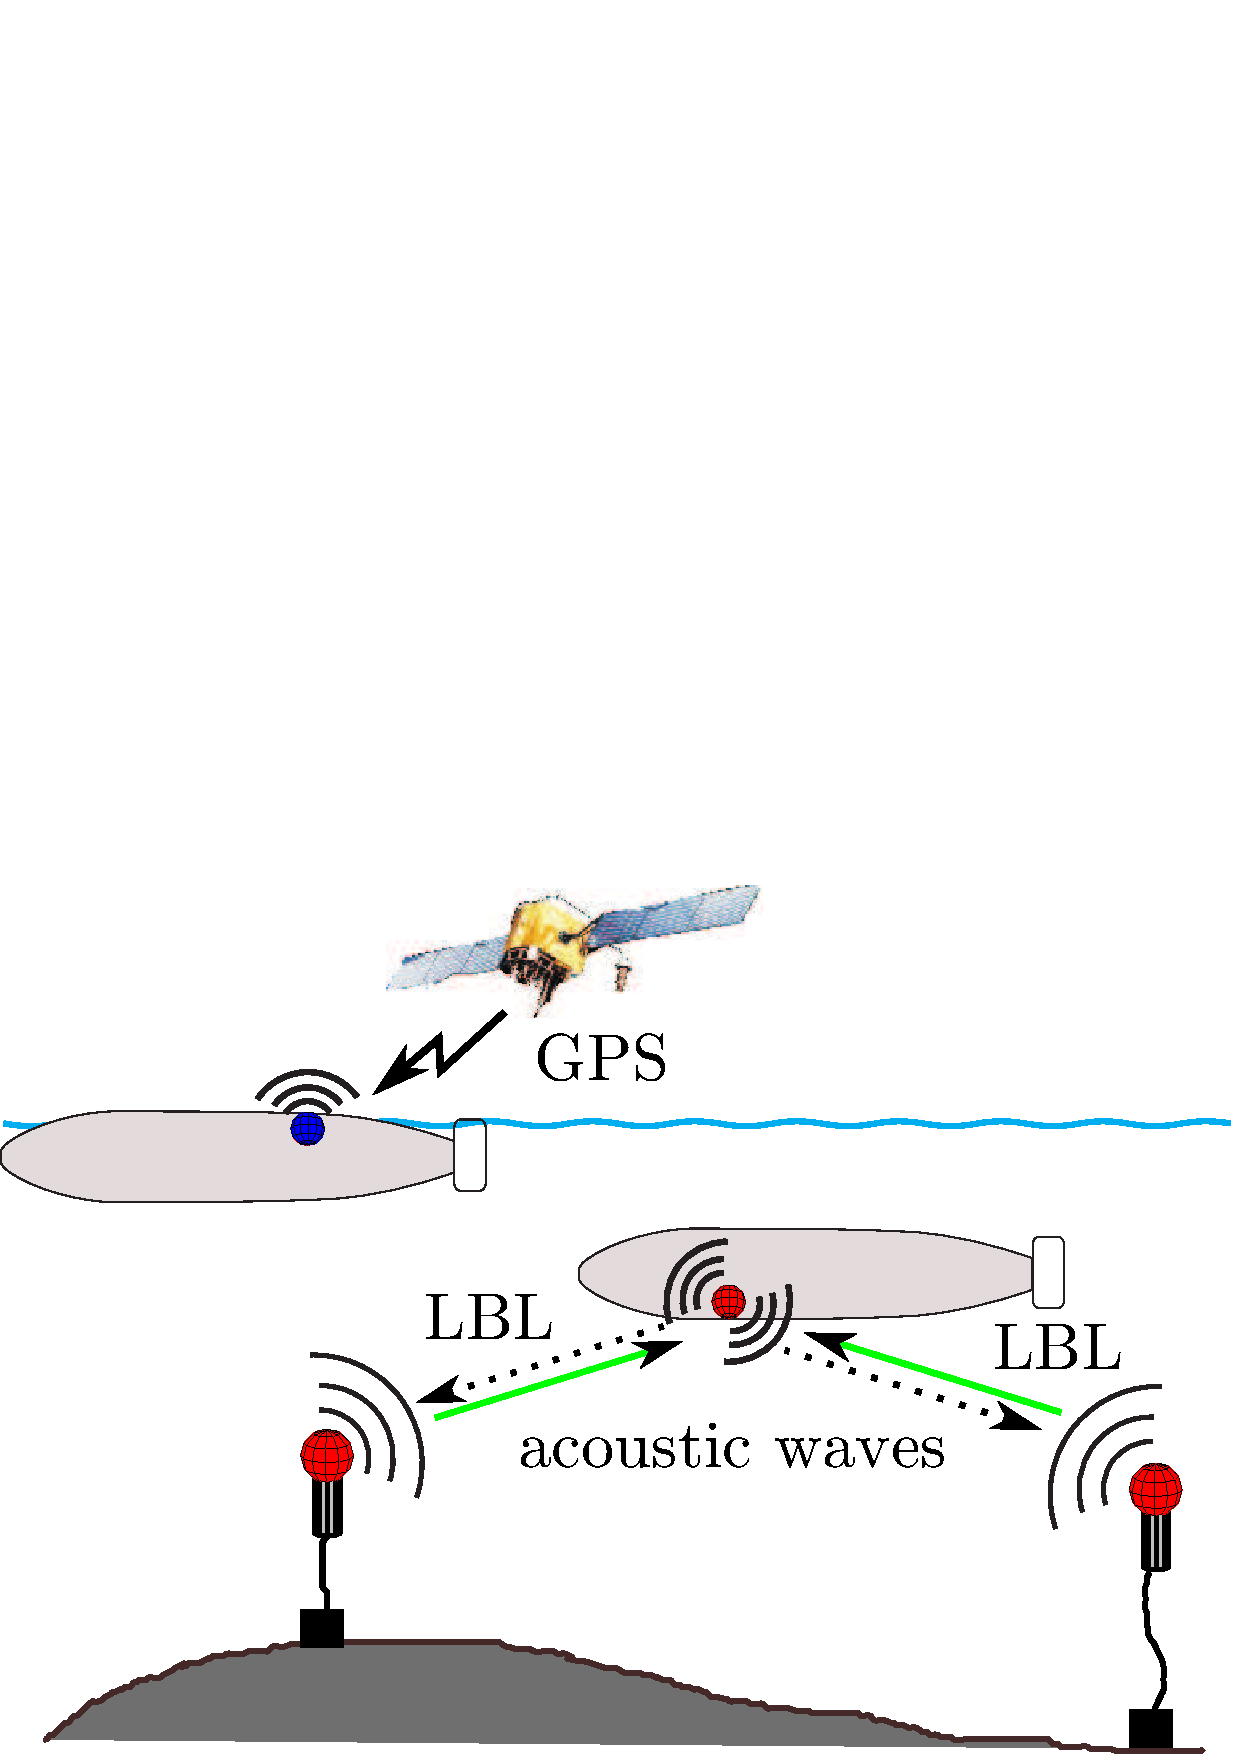
\includegraphics[width=0.7\linewidth]{fig/lbl-gps.pdf}
	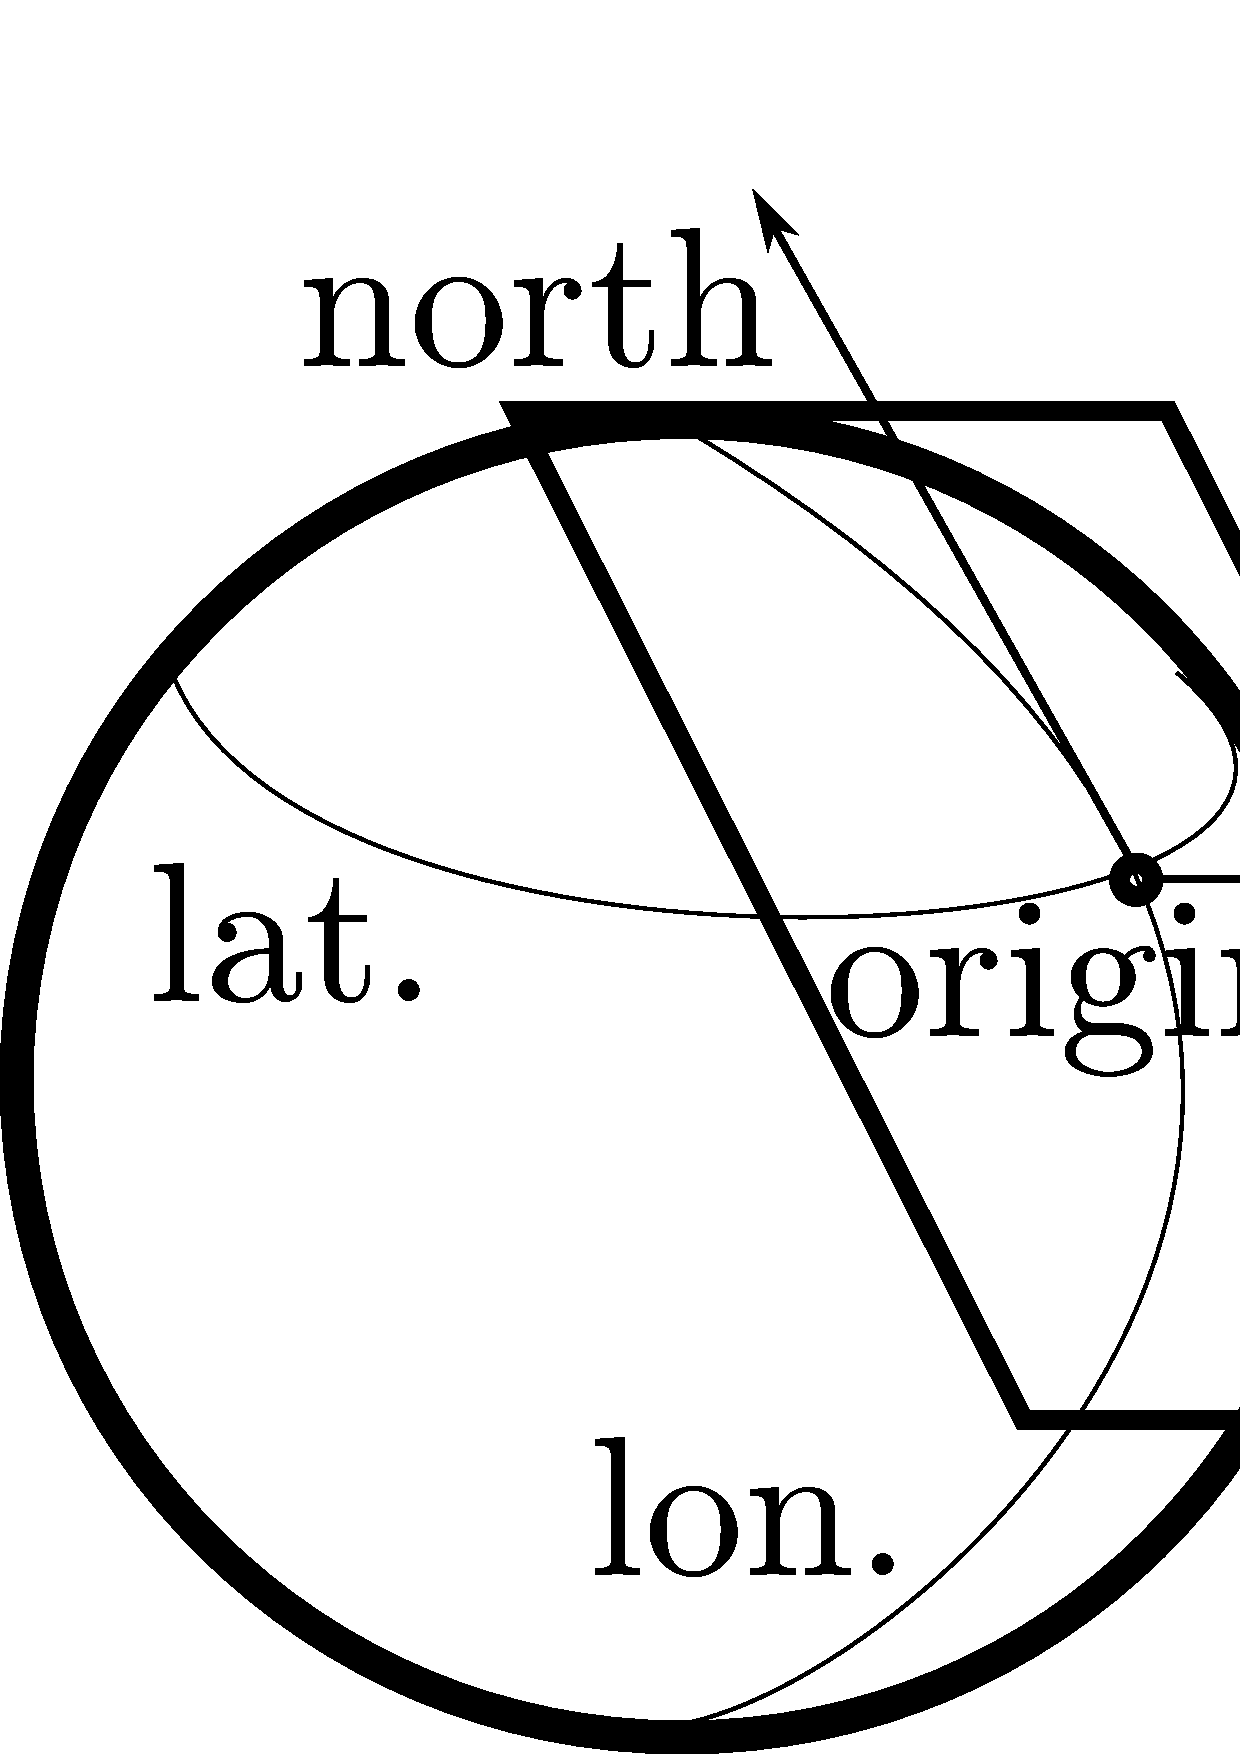
\includegraphics[width=0.28\linewidth]{fig/positioning.pdf}	
	\end{block}

\end{columns}

%\begin{columns}[t]
%	\column{.3\textwidth}
%	\begin{block}{}
%	\end{block}
%	
%\end{columns}
\end{frame}
